\documentclass{beamer}
\usepackage[T1]{fontenc}
\usepackage[utf8]{inputenc}
\usepackage{amsmath}
\usepackage{amssymb}
\usepackage{tikz}
\usepackage{graphicx}
\usetikzlibrary{automata,positioning}

\title{The Reverse of a Regular Language is Regular}
\author{Tanisha Ahuja \and Natasha}
\institute{COMP 382}
\date{\today}

\begin{document}

\begin{frame}
\titlepage
\end{frame}

\begin{frame}{Problem Statement}
Given any DFA $M$, prove that:
\[ (L(M))^R = \{ w^R \mid w \in L(M) \} \]
is regular.
\end{frame}

\begin{frame}{Key Idea}
\begin{itemize}
    \item Convert DFA to NFA by reversing transitions
    \item Swap start and accept states
    \item The resulting NFA accepts the reverse language
    \item Since NFAs recognize regular languages, we're done!
\end{itemize}
\end{frame}

\begin{frame}{Construction}
Given DFA $M = (Q, \Sigma, \delta, q_0, F)$:
\begin{itemize}
    \item Create NFA $M' = (Q, \Sigma, \delta', F, \{q_0\})$
    \item For each transition $\delta(q,a) = p$ in $M$
    \item Add transition $\delta'(p,a) = q$ in $M'$
\end{itemize}
\end{frame}

\begin{frame}{Example - Original DFA}
\begin{center}
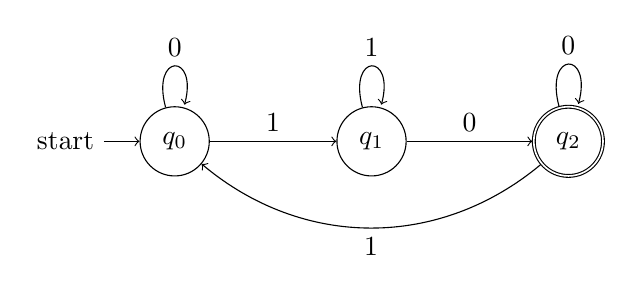
\begin{tikzpicture}[auto,node distance=2.5cm]
    % Original DFA
    \node[state,initial] (q0) {$q_0$};
    \node[state,right of=q0] (q1) {$q_1$};
    \node[state,accepting,right of=q1] (q2) {$q_2$};
    
    \path[->]
        (q0) edge[loop above] node{0} (q0)
        (q0) edge[above] node{1} (q1)
        (q1) edge[loop above] node{1} (q1)  % Added q1 self-loop with 1
        (q1) edge[above] node{0} (q2)
        (q2) edge[loop above] node{0} (q2)  % Added q2 self-loop with 0
        (q2) edge[bend left=40] node{1} (q0);
\end{tikzpicture}
\end{center}
Example string: 10110 \\
Path: $q_0 \xrightarrow{1} q_1 \xrightarrow{0} q_2 \xrightarrow{1} q_0 \xrightarrow{1} q_1 \xrightarrow{0} q_2$
\end{frame}

\begin{frame}{Example - Reversed NFA}
\begin{center}
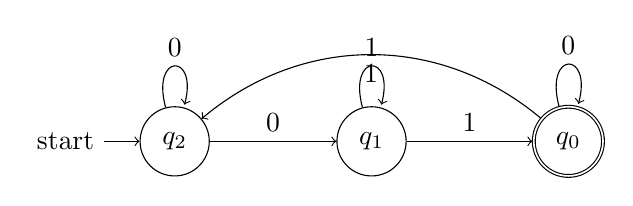
\begin{tikzpicture}[auto,node distance=2.5cm]
    % Reversed NFA
    \node[state,initial] (q2) {$q_2$};
    \node[state,right of=q2] (q1) {$q_1$};
    \node[state,accepting,right of=q1] (q0) {$q_0$};
    
    \path[->]
        (q2) edge[loop above] node{0} (q2)  % Added q2 self-loop with 0
        (q2) edge[above] node{0} (q1)
        (q1) edge[loop above] node{1} (q1)  % Added q1 self-loop with 1
        (q1) edge[above] node{1} (q0)
        (q0) edge[loop above] node{0} (q0)
        (q0) edge[bend right=40] node{1} (q2);
\end{tikzpicture}
\end{center}
Example string (reversed): 01101 \\
Path: $q_2 \xrightarrow{0} q_1 \xrightarrow{1} q_0 \xrightarrow{1} q_0 \xrightarrow{0} q_1 \xrightarrow{1} q_0$
\end{frame}

\begin{frame}{Proof Sketch}
\begin{itemize}
    \item If $w = a_1a_2...a_n$ is accepted by $M$
    \item Then $w^R = a_n...a_2a_1$ is accepted by $M'$
    \item Because we can follow the path in reverse
    \item Start states become accept states
    \item Accept states become start states
\end{itemize}
\end{frame}

\begin{frame}{References}
\begin{itemize}
    \item Sipser, M. (2012). Introduction to the Theory of Computation
    \item Hopcroft, J. E., et al. (2006). Introduction to Automata Theory
\end{itemize}
\end{frame}

\end{document}\end{document}
